\documentclass[12pt]{article}

% Packages
\usepackage{amsmath, amssymb}
\usepackage{graphicx}
\usepackage{geometry}
\usepackage[backend=biber, style=apa]{biblatex} % Use biblatex with biber
\usepackage{wrapfig}
\usepackage{hyperref}


% Page layout
\geometry{a4paper, margin=1in}

% Bibliography file
\addbibresource{references.bib} % Specify the .bib file

% Title and Author
\title{Title of the Paper}
\author{Author Name}
\date{\today}

% ------------------------------------------------------------------------------
% Document
\begin{document}

\maketitle
% 1. Executive Summary
\section*{1. Executive Summary (max half page)}
% Your summary here.

% 2. Introduction
\section*{2. Introduction (about one page)}
\subsection*{(a) Cause and impact of economic fluctuations}
% Content here.

\subsection*{(b) Consequences for economy and why policy should act}
% Content here.

\subsection*{(c) Brief overview of suggested policy}
% Content here.



% ------------------------------------------------------------------------
% THEO ------------------------
% ------------------------------------------------------------------------

% 3. Bird’s Eye View of the Model
\section*{3. Bird’s Eye View of the Model (about two pages)}

\subsection*{(a) Outline of the Model Structure (graphical and verbal, no equations)}
% Content here (include figure environment if needed).

\subsection*{(b) Policy Structure of the Model (main equations)}
% Content here (use align or equation environments).

\subsection*{(c) Calibration of the Model}
% Content here.

\newpage
% ------------------------------------------------------------------------
%  JAKUB -------------------------------
% ------------------------------------------------------------------------

% 4. Benchmark Model Analysis
\section*{4. Benchmark Model Analysis (about two pages)}

As our scenario requires that the Central Bank adopts a money supply target, we adjust the benchmark model to a monetary policy rule with the following specification: 

\begin{equation}
    \frac{M_t}{M_{t-1}} = \Big(\frac{MC_{t}}{\bar{MC}}\Big)^{\theta_{MC}} \Big(\frac{1+\pi_{t}}{1+ \bar \pi}\Big)^{\theta_{\pi}}
\end{equation}

Moreover, it seems natural, that the $MC$ shock should enter the model through the Phillips curve. That is because the curve represents the pricing decision rule of the intermediate companies, and so it will most accurately represent their reaction to an increase in marginal costs.

\subsection*{(a) How does the shock lead to economic fluctuations (baseline scenario)?}

These two assumptions lead to the fact that in the period following the shock, intermediate firms will adjust their prices and revise their hiring decisions. The economic intuition behind this is that an increase in marginal costs, decreases the markup of the firm which then chooses to adjust its prices. As adjustment is costly (due to $\kappa$), the firms will raise their prices less than the increase in marginal costs. In turn, higher prices, cause a decrease in demand for the aggregate product, therefore prompting the firms to decrease output. At the same time, the higher marginal costs imply that the companies choose to hire less labour and capital, as it becomes more costly. Finally, real wages and the real rental rate of capital fall, as \dots\ \textit{finish} \dots\ \textbf{Note: Check my reasoning here.}

Furthermore, the $MC_t$ feeds into firms' expectations about the future. When firms choose to set their prices for $t$, they trade off increasing their prices today and in the future. If the shock is expected to be persistent, firms may choose to increase their prices by less in $t$ and choose to keep increasing them slowly over time. 

The firm's pricing decision is also important for the future, as it is used as a benchmark relative to which they set their next period's prices. If prices are set high in period $t$, \textbf{does it increase the costs of raising the prices later on??? I don't think so}.

Over time, as no more shocks happen, firms are able to arrive back at their target markup and therefore the economy is able to come back to the steady state inflation rate.\ \textbf{Expand on this part.}

\begin{figure}
    \caption{Impulse response functions of observable variables}\label{fig:obs_var_taylor}
    \centering
    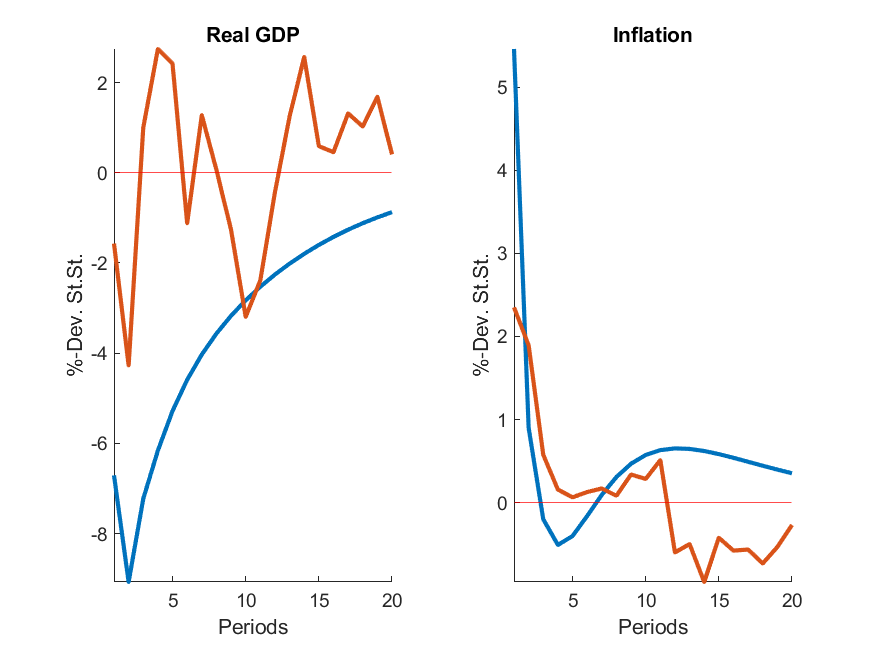
\includegraphics[width=0.7\textwidth]{../matlab_base/output/irf_gdp_taylor.png}
\end{figure}

\textbf{I THINK THAT THIS IS ALSO WHERE WE ADD OUR IMPULSE RESPONSE FUNCTIONS AS DESCRIBED IN THE INSTRUCTIONS!!!!}

% describe the short run as well as the path back to the steady state. 
\subsection*{(b) What is the idea behind the implemented policy (current policy scenario)?}

At the same time, in an effort to smooth out the path of the economy, the central bank will adjust the money supply to increase the purchasing power of the households and counter the shocks. By following the Taylor-like monetary policy rule, it will increase the money supply in order to match the inflation and marginal cost gaps of the economy in an effort to achieve price stability. As the bank intervention will increase the money stock of the households, it will allow it to consume more goods and therefore counter the drop in output that the economy experiences.\ \textbf{Think carefully about this, what is the ideal policy rule and how to actually best achieve price stability, what should the central bank target?}

\newpage
% 5. Counterfactual Policies
\section*{5. Counterfactual Policies (about two pages)}
\subsection*{(a) More or less of the same policy (different coefficients)?}
% Content here.

\subsection*{(b) Alternative policy (different targets)?}
% Content here.

% -------------------------------------------------------
%                       NOTES
% -------------------------------------------------------
% - try adding in the labour supply target instead of MC
% - think about implementing alternative inflation target (0.03)
% - think about alternative monetary policy rules 
% -  fiscal instead of monetary as a counter-factual?




% -------------------------------------------------------


% 6. Policy Recommendation and Discussion
\section*{6. Policy Recommendation and Discussion (about one page)}
\subsection*{(a) Give a recommendation on policy based on your simulations.}
% Content here.

\subsection*{(b) Should policy have taken a different path?}
% Content here.

\subsection*{(c) Do your results confirm or conflict with your perception about optimal policy? Discuss how.}
% Content here.
% \printbibliography() % Print the bibliography

\end{document}